\section{Methodology}
\label{ch:methodology}

Having established necessary background knowledge in the previous chapter,
the experiments of this work can be introduced.
This chapter will first examine prior work in the area of tweet engagement
prediction (ch.~\ref{sec:prior_work}), before outlining limitations of this
research.
Afterwards, structure and aim of the developed models will be explained in general (ch.~\ref{sec:approach}).
Chapter~\ref{sec:data_collection} presents data used in this thesis.
The final subsection describes the infrastructure, i.e., software and hardware,
which was used to develop deep learning models.

\section{Prior Work}
\label{sec:prior_work}

This section lists previous work in tweet engagement prediction, starting with
general retweet research and then introducing models that cope with different
kinds of prediction problems.
Predictive models in this area are largely focused on retweet prediction.
This can be explained by the sharing effect of retweeting, which can be interpreted
as information diffusion, a highly researched area in social network analysis.
Previously developed models were roughly classified according to their problem type.

\paragraph{General retweet research}

General research on the act of retweeting offers intuitions about the mechanism
and gives way for feature ideas for machine learning models.
Boyd et al.~\cite{Golder} examine conversational aspects of retweeting and
compare the mechanism to other behavioral conventions on the Twitter platform,
namely mentions and hashtags.
Where mentions constitute a form of direct messaging and hashtags enable
communication around specific topics, retweeting is a form of information
diffusion and participating in conversations without actively contributing.
Furthermore, the authors identify motivations for retweeting, e.g., showing
presence as a listener or validating a tweet.
According to their examination, the most commonly retweeted content is
time-sensitive, e.g., breaking news.
Factors influencing retweetability have also been the subject of other work.
Features are often separated into content and contextual features.
Among content features, the use of URLs and hashtags has been shown to be
positively correlated with retweetability, especially for URLs that are seen
as particularly interesting by human respondents~\cite{Suh}.
Contextual features comprise all factors related to the source user, his
following and activitiy on the platform.
The number of followers and friends, as well as account age have positive
effects on retweetability.
Moreover, past activity, e.g., tweet frequency was shown to not be significantly
influential~\cite{Bakshy2011, Suh}.
Retweeting has also been analyzed in temporal fashion, mainly through the use
retweet graphs which constitute representations of cascades.
Kwak et al.~\cite{Kwak2010} show that most retweeting acts occur in the first
and second degree network of the source user.
Additionally, most retweeting happens in a concise time frame.
Namely, 50 \% of retweets take place within one hour, 75 \% within a day and more
than 90 \% in one month after tweet creation.

\paragraph{Retweet probability prediction}

Retweet probability prediction refers to the problem of forecasting the
probability that a given destination user will retweet a specific tweet of
the source user.
This problem has drawn interest from the research community in the past, and
multiple models have been developed for this purpose.
First models only used very simple features like tweet words, identity of the
source user and the number of his followers and friends~\cite{Zaman2010}.
Other work focuses on content features, which can be divided into two separate
categories.
Low-level features include used words, the number of hashtags, URLs and mentions,
as well as usage of positive and negative terms according to predefined word 
classification.
High-level features on the other hand describe more complex features such as
the association to topics or sentiments.
Naveed et al.~\cite{Naveed2011} develop a logistic regression model using
both types of features and find that tweets regarding more general and 
negatively connoted topics have a higher probability of being retweeted.
More complex features are included by Peng et al.~\cite{Peng2011},
who employ conditional random fields for their predictive model.
The authors include content features such as topic similarity of a tweet with 
interests of the source user and his audience.
In addition, activity data is used, e.g., tweet frequencies of user and
followers around specific times.
A new set of features involves the relationship between source and destination
user, i.e., the number of mutual followers, friends and mentions.
It is shown that user features are most helpful for the prediction of
retweet probability.
Lee et al.~\cite{Lee2014} go a step further and try to identify the most
effective message propagator for a given tweet.
They rely on a rich set of manually crafted features around personality and activity data
and employ different machine learning models, e.g., random forest, logistic
regression and support vector machines.

\paragraph{Classification approaches}

As introduced in ch.~\ref{sub:dl_terminology}, classification models learn a
mapping between inputs and predefined sets of outputs.
A model employing an output variable with exactly two possible values is referred
to as a \textit{binary classification model}.
This approach can be used for retweet prediction approach, namely if the goal
of the model is to simply determine whether a given tweet will be retweeted
or not.
So-called \textit{multi-class classification models} aim to deliver a more
precise prediction regarding the number of retweets.
Hong et al.~\cite{Hong2011} have developed both types of models in their work
using a logistic regression approach.
Whereas the binary classification model shows promising results, the multi-class
model only performs well for predicting retweet counts of 0 and larger than
10,000.
Classes inbetween these two extremes are predicted with much lower accuracy.
Another binary classification model was introduced by Petrovic et al.~\cite{Petrovic2011}
who focus on the creation a deployable model.
This leads to the utilization of simple content and contextual features, as described
in the above paragraph.
They find that contextual features, especially regarding the source user,
have higher predictive power than tweet features.
The models achieve accuracy metrics between 70 and 80 \% on different tasks,
which is not significantly different from recorded human performance.

\paragraph{Regression approaches}

Regression models aim to predict a specific value for given inputs.
For retweet prediction this refers to forecasting a numerical value for the
eventual retweet count.
Since the retweet process after tweet creation has no preset determination date, general assumptions
about the temporal retweet distribution have to be made when building
regression models.
Kupavskii et al.~\cite{Kupavskii2012} try to predict the eventual size of the
retweet cascade, i.e., the graph whose vertices represent retweeting users.
At the time, this constituted a novel task which enables two distinct predictions:
one at the initial point of tweet creation, the second after a short
time of observing the retweet cascade.
Obviously, the second prediction can be made using more information about the
initial message spread.
The authors employ a gradient boosted decision tree based on standard content
features (see above paragraphs).
Additionally, they take retweet ratios of creating user and followers into
account and precalculate PageRank statistics for all considered users on a
separate data set of retweet graphs.
Thus, they gain more insights into retweeting behavior of users in their data
set.
As expected, observing retweet cascades for some time improves the quality
of their prediction considerably.
A comparable approach is used by Zaman et al.~\cite{Zaman2014}, whose work
examines retweet time series for 52 manually chosen tweets.
They find that the median of all retweets occurs between four minutes and three
hours after tweet creation.
In addition, they develop a Bayesian model for evaluating the retweet graph
which is able to utilize parts of the time series data to improve its
prediction.
The model outperforms a linear regression baseline using only
the follower count as input data.
Moreover, the prediction becomes more precise the more time series data is utilized
as an input.

Having established this line of prior research, the approaches used in this
work can now be described.


\subsection{Approach}
\label{sec:approach}

The introduction to this thesis stated its main objective, namely the
development of a deployable stand-alone model for precisely predicting tweet
engagement metrics.
As previously elaborated, `deployable' in this context stands for the practical
applicability of the model.
The term `stand-alone' denotes the requirement of solely relying
on data that stems directly from tweet objects of the public Twitter interface.
Not being dependent on additional data would enable the system to be applicable
in a streaming setting.
Furthermore, predicted engagement metrics should incorporate both eventual
retweet and favorite counts.
This section comprises three parts.
Firstly, limitations of the previously described prior work with regard to the
stated objective are outlined.
Secondly, the experiments conducted in this thesis are introduced.
Finally, necessary assumptions for the developed models are stated and justified.

\subsubsection{Limitations of prior research}

This thesis aims to develop deep learning models for predicting tweet
engagement.
Employing deep learning should help to overcome several limitations of prior
work in this research area (see ch.~\ref{sub:meth_prior_work}), which will be listed in the following.
Some of the described models rely on complex, manually crafted features, e.g.,
activity, topic similarity and relationship features.
These often require additional data and excessive preprocessing, in some cases
even precalculated models on separate data sets.
This stands in contrast to the ad-hoc processing requirement in the objective.
The hypothesis of this work is that these features can be omitted or
learned intrinsically by deep neural networks.
Manual feature creation is necessary for machine learning models like logistic
regression or decision trees that are less capable of creating own feature
representations.
Deep neural networks achieve higher representational capability by effectively
stacking non-linear modules which learn discrete features according to the problem at
hand~\cite{LeCun2015}.
One objective for this thesis is an accurate prediction of the eventual popularity
of tweets.
Previous models mostly focus on probability prediction or binary classification
which is insufficient to meet this objective.
Furthermore, less complex models have not shown good performance in the multi-class
classification setting, only showing good accuracy for extreme cases.
This work tries to overcome this limitation by employing deep models on diverse
data sets with varying class distributions.
Following this approach should also conquer biases in the collected data.
In previous research, data sets were often collected around a single topic or
trend, sometimes even handpicked~\cite{Zaman2014}.
Both models that apply predictive models in a regression setting are dependent
on some form of time-series observation of the retweet graph, which is not adequate for
an accurate prediction about future engagement at the time of tweet creation.
In this work, models are able to make real-time predictions, i.e., it could
be possible to deploy them in an application that is fed data from the Twitter
Streaming API~\footnote{\url{https://developer.twitter.com/en/docs/tweets/filter-realtime/overview/powertrack-api}}.
An additional feature of models in this work is their capability to predict both
number of retweets and favorites.

\subsubsection{Developed models}

Models developed in this thesis make use of content and contextual features,
inspired by previous work in this field.
Since the models only rely on tweet objects from the Twitter API, contextual
features are mainly limited to information about the source user~\footnote{\url{https://developer.twitter.com/en/docs/tweets/data-dictionary/overview/intro-to-tweet-json}}.
In contrast to previous model, sophisticated deep learning models should allow
more precise processing of tweet content, particularly because deep neural networks
show good performance on natural language processing tasks (see ch.~\ref{sub:dl_app_nlp}).
In summary, the deep models are fed both structured and unstructured data.
Here, structured data represents inputs that could easily be stored in
tabular format, e.g., a relational database.
Examples for these features include number of hashtags and URLs on the content
side, as well as follower count and account age on the contextual side.
The actual tweet content can be seen as unstructured data, due to its variation
in length and manifestation.

\begin{figure}[h]
  \centering
  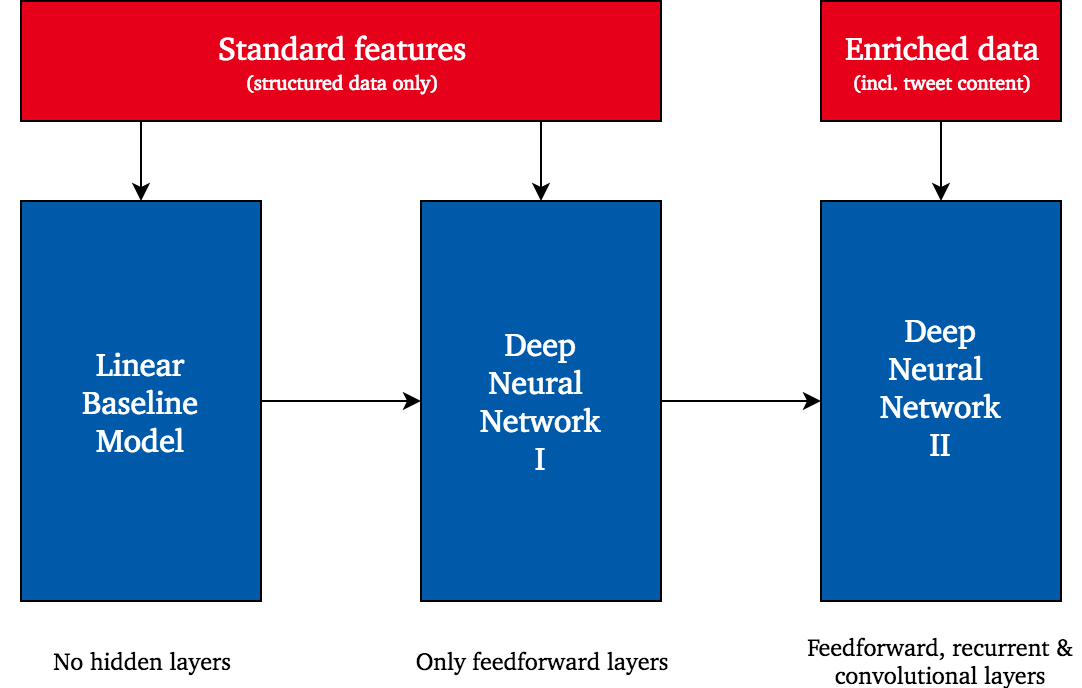
\includegraphics[height=9cm]{img/model_summary}
  \caption{Summary of developed models}
\label{fig:model_summary}
\end{figure}

Fig.~\ref{fig:model_summary} sums up the intended model evolution for this thesis.
Each model will be used in both a regression and multi-class classification
setting, producing separate predictions for retweet and favorite counts.
In order to enable comparisons, a linear baseline model will be created first.
This model will be trained solely using structured data.
In their essence, these models represent linear and logistic regression models
respectively.
Afterwards, a deep neural network is trained on the same structured data sets.
This model employs standard feed-forward layers (see ch.~\ref{sub:dl_concepts}),
which enables more complex input representations and hence more accurate
predictive outputs.
The final model is trained using enriched, i.e., structured and unstructured,
input data and more sophisticated layer architectures.
Both convolutional and recurrent layers are deployed in order to derive more
powerful features from the tweet content. 
Including textual input data requires additional preprocessing steps which aim
to transform words into floating-point numbers.
However, these additional steps do not hinder the practical applicability
of the model since they are not costly computation-wise.

\subsubsection{Assumptions}

This work relies on the assumption that most retweeting occurs in a short time
span after tweet creation.
Following this assumption, retweet and favorite counts can be approximated
to be precise estimates of the tweet engagement one month after the initial
creation.
This important assumption can be justified by research which conducts analysis
on large tweet data sets.
The overall conclusion of such research is that half of retweeting occurs within
hours, and more than 90 \% within one month after tweet publication~\cite{Kwak2010, Kupavskii2012, Zaman2014}.

Having established intended experiments for this work, the concluding section
in this methodology chapter will describe the examined data sets and the
collection process.


\subsection{Data}
\label{sec:data_collection}

The main goal of this thesis regarding the examined data is to have diverse
data sets from users for which engagement prediction has practical relevance.
The diversity requirement mainly comprises different retweet distributions
so that the model performance can evaluated in a generalized manner.
Predicting the popularity of tweets is relevant for all individuals and
organizations that somehow rely on social media marketing or customer support.
Therefore, the collected data sets include data from public figures and
companies, most of whom actively maintain a Twitter account.
The selected accounts were separated into three groups and saved as Twitter lists
in the author's profile (see Appendix).
For each of the three groups, all tweets from January to August 2017 were
fetched from the public Twitter API~\footnote{\url{https://developer.twitter.com/en/docs/tweets/timelines/api-reference/get-statuses-user_timeline.html}}.
Afterwards, retweets that the specified users made were excluded since their
engagement statistics are not related to their accounts, but the users who
originally created their tweets.
In summary, the final data sets include all status updates and quotes from the
specified users in the given time frame.
It was ensured that all collected tweets were older than one month 
at the time of retrieval.
As mentioned in the previous section, the third stage of model development
for this thesis aims to extract meaningful features from the raw tweet content.
This typically requires a huge number of data points, so that popular NLP benchmark
data set for similar tasks, e.g., sentiment analysis, usually contain more than
a million labeled training examples~\footcite{Go2009}.
In order to account for these massive data requirements, an additional data set was
collected, which includes all tweets from the aforementioned user groups over
the course of two years.

\begin{table}
\begin{tabular}{lllr}
\toprule
  Accounts & Total accounts & Time frame & Total tweets \\
\midrule
  Fortune 500 companies & 441 & 1/2017 - 8/2017 & 254,059 \\
  US Governors and Senators & 162 & 1/2017 -  8/2017 & 94,919 \\
  Celebrities & 170 & 1/2017 - 8/2017 & 46,986 \\
  Companies, politicians \& celebrities & 773 & 1/2016 - 12/2017 & 863,004 \\
\bottomrule
\end{tabular}
\caption{Summary of collected data sets}
\label{tab:dataset_summary}
\end{table}

Table~\ref{tab:dataset_summary} sums up all data sets used for the purpose of
this work.
The first data set comprises all Twitter accounts from \textit{Fortune 500}
companies in 2017~\footnote{\url{http://fortune.com/fortune500/}}.
All in all, 441 out of 500 companies operate a Twitter presence, which accounted
for a total of 254,059 tweets in the evaluated period.
The second user group includes all Twitter accounts of US Senators~\footnote{\url{https://twitter.com/cspan/lists/senators}} and Governors~\footnote{\url{https://twitter.com/cspan/lists/governors}}
as of October 2017 which were derived from Twitter lists by the television
network \textit{C-SPAN}.
From January to August 2017, 162 politicians created a total of 94,919 tweets.
The smallest data set stems from celebrities, namely the \textit{Forbes Highest-Paid
Athletes 2017}~\footnote{\url{https://www.forbes.com/sites/kurtbadenhausen/2017/06/15/full-list-the-worlds-highest-paid-athletes-2017}}, \textit{Forbes Highest-Paid Actors and Actresses 2017}~\footnote{\url{https://www.forbes.com/sites/natalierobehmed/2017/08/22/full-list-the-worlds-highest-paid-actors-and-actresses-2017}} and
\textit{Forbes Highest-Paid Celebrities 2017}~\footnote{\url{https://www.forbes.com/sites/zackomalleygreenburg/2017/06/12/full-list-the-worlds-highest-paid-celebrities-2017}}.
The derived data set contains 46,986 tweets from 170 accounts.
Over the course of 2016 and 2017, all users combined accounted for a total
of 863,004 tweets which comprise the additional data set.
It has to be mentioned that company tweets account for an unproportionally high
percentage (around 60\%) of all tweets in this data sets, simply due to greater
total of accounts from this group.

Examining deep neural network performance on differently sized data sets should
enable to draw conclusion about data requirements for the particular problem
of engagement prediction.
Descriptive statistics for all data sets can be found in ch.~\ref{sec:dda}.


\subsection{Infrastructure}
\label{sec:infrastructure}

The experiments in this thesis were conducted using infrastructure suitable
to handle complex computations and large data sets.
This section will describe hardware (ch.~\ref{sub:meth_hardware}) and software
(ch.~\ref{sub:meth_software }) which was applied to the problem of tweet
engagement prediction.

\subsubsection{Hardware}
\label{sub:meth_hardware}

As stated in Chapter~\ref{sub:dl_drivers}, training deep neural networks
typically requires the parallel computing power of graphics processors.
In addition, large data files need to be stored and processed.
Cloud environments are well suited for these tasks, since they enable on-demand 
access to specialized hardware.
\textit{Amazon Web Services} was chosen as primary infrastructure provider for 
work on this thesis, mainly due to familiarity and a broad palette of offered
solutions.
Raw, unfiltered data files containing tweet and author information were stored
on an \textit{Amazon S3}\footnote{\url{https://aws.amazon.com/s3/}} instance,
which could be accessed programmatically or via the management console.
After filtering retweets and extracting features, the prepared data sets could
permanently be saved on the respective processing instance for improved
accessibility.
Training of deep learning models was undertaken on an \textit{Amazon EC2}\footnote{\url{https://aws.amazon.com/ec2/}}
instance.
Namely, the specification \textit{p2.xlarge} was chosen in order to train models
on a GPU.
These instances employ a \textit{NVIDIA K80} GPU with 12GB of memory and 2,496
processing cores.
Moreover, p2.xlarge machines possess 61GB of memory and four CPU cores.

\subsubsection{Software}
\label{sub:meth_software}

All model development was conducted using the \textit{Python}\footnote{\url{https://www.python.org/}} programming language,
since it offers extensive and well-docomented libraries for data analysis and numerical computation.
\textit{Jupyter notebooks}\footnote{\url{http://jupyter.org/}} were used as development environment, because
of their capability to combine code, visualizations and documentation in a single
document.
Conducting experiments in notebooks proved to increase reproducibility of results
and overall project organization.
Reusable functionality tested in notebooks was often transferred to Python
modules.

\outline{Development environment: Jupyter notebooks (+ self-written Python modules)}

\outline{Data collection: python-twitter library}
\outline{Possible alternatives: using API directly, wrangling with JSON (not as convenient)}

\outline{Data analysis and wrangling: pandas, numpy, matplotlib, scikit-learn}

\outline{Model training: Keras (high-level API) with Theano backend (low-level: cudNN, CUDA)}
\outline{Possible alternatives: TensorFlow, PyTorch (not as familiar to author)}

This section about infrastructure concludes the methodology chapter.
The upcoming chapter will describe results of experiments undertaken in this
thesis.

